\chapter{Relativistic Kinematics}\label{ch:b3:relativistic-kinematics}

Cosmic rays striking the upper atmosphere create muons fifteen
kilometres up --- unstable particles that live, on average, two
microseconds. Two microseconds at nearly the speed of light is
six hundred metres; yet muon detectors at sea level click steadily,
counting particles that have crossed twenty times their allotted
range. The resolution of this paradox is not a detail of particle
physics but a revision of the concepts beneath all of physics: time
elapses differently for the moving muon than for us, and distances
shrink along its motion. This chapter builds that revision --- special
relativity (Einstein, 1905) --- from its two postulates: the laws of
physics are the same in every \omterm{thm:b3:relativistic-kinematics:postulates}{inertial frame}, and light in vacuum has
the same speed in all of them. Everything else follows by honest
kinematics: the entanglement of space with time in the \omterm{thm:b3:relativistic-kinematics:lorentz}{Lorentz
transformation}, the dilation of time, the contraction of lengths, the
new rule for adding velocities, and the geometry --- spacetime and its
invariant interval --- in which all of it becomes as natural as
rotations.

\section{Two postulates against absolute time}

\begin{remark}[Where the conflict comes from]\label{rem:b3:relativistic-kinematics:conflict}
Mechanics has always had a relativity principle: inside a smoothly
sailing ship, no experiment with balls and pendulums betrays the
motion (Galileo), and Newton's laws hold in every \emph{\omterm{thm:b3:relativistic-kinematics:postulates}{inertial
frame}}, the frames in motion at constant velocity relative to one
another. But the electromagnetism of the Year 2 volume derives a
definite speed for light, $c = 1/\sqrt{\varepsilon_0\mu_0} =
\qty{3.00e8}{m/s}$, from constants of nature, with no mention of who
measures it --- and experiments agree: the speed of starlight arriving
at the moving Earth, measured across the seasons, never varies
(Michelson and Morley, 1887, and every successor since). Galilean
kinematics, in which velocities add, cannot digest a speed that is the
same for everyone. Something has to give, and it is our assumption
that time and \omterm{def:b3:relativistic-kinematics:event}{simultaneity} are absolute.
\end{remark}

\begin{theorem}[The postulates of special relativity]\label{thm:b3:relativistic-kinematics:postulates}
\index{relativity!postulates}\index{inertial frame}
\emph{(i) Relativity:} the laws of physics take the same form in every
\omterm{thm:b3:relativistic-kinematics:postulates}{inertial frame}; no experiment distinguishes rest from uniform motion.
\emph{(ii) Light:} light in vacuum propagates at the same speed $c$ in
every \omterm{thm:b3:relativistic-kinematics:postulates}{inertial frame}, whatever the motion of the source or the
observer.
\end{theorem}
\admitted

\begin{definition}[Events and simultaneity]\label{def:b3:relativistic-kinematics:event}
\index{event}\index{simultaneity}
An \emph{event} is a point occurrence: a definite place \emph{and} a
definite instant --- a spark, a detector click, a decay. Each \omterm{thm:b3:relativistic-kinematics:postulates}{inertial
frame} assigns an event its coordinates $(t, x, y, z)$, using rulers at
rest in the frame and synchronised clocks distributed through it. Two
events are \emph{simultaneous in a frame} when that frame's clocks
assign them the same $t$ --- and the first casualty of the postulates
is that this notion depends on the frame.
\end{definition}

\begin{example}[The train and the two lightning bolts]\label{ex:b3:relativistic-kinematics:train}
Lightning strikes both ends of a fast train, leaving marks on train
and track. For the observer on the ground, midway between the marks,
the two flashes arrive together: the strikes were simultaneous for
her. The passenger seated at the train's midpoint, however, is moving
toward one flash and away from the other; travelling at $c$ in his
frame too, the forward flash reaches him first --- and since he sits
equidistant from the two marks \emph{on the train}, he must conclude
the forward strike happened \emph{earlier}. Neither is wrong:
\omterm{def:b3:relativistic-kinematics:event}{simultaneity} of separated \omterm{def:b3:relativistic-kinematics:event}{events} is not a fact about the world but
about the frame. Every relativistic ``paradox'' dissolves here.
\end{example}

\begin{omfigure}
\begin{tikzpicture}[font=\small, >=Stealth]
  % ground view
  \begin{scope}
    \draw[thick] (-0.3,0) -- (10.3,0);
    \fill[omDef!18, draw=omDef, thick, rounded corners=2pt] (1.4,0.15) rectangle (8.6,1.05);
    \foreach \x in {2.2,3.4,4.6,5.8,7.0} \draw[omDef] (\x,0.35) rectangle (\x+0.7,0.85);
    \draw[->, very thick] (8.9,0.6) -- (9.9,0.6) node[right] {$v$};
    \node[omExo] at (1.4,1.75) {\Large$\downarrow$};
    \node[omExo] at (8.6,1.75) {\Large$\downarrow$};
    \node[omExo, font=\footnotesize] at (1.4,2.15) {strike A};
    \node[omExo, font=\footnotesize] at (8.6,2.15) {strike B};
    \fill (5,-0.02) circle (2pt);
    \node[font=\footnotesize] at (5,-0.4) {ground observer, midway};
    \fill[omThm] (5,1.22) circle (2pt);
    \node[omThm, font=\footnotesize] at (5.1,1.55) {passenger, mid-train};
  \end{scope}
\end{tikzpicture}

{\small Two strikes marking both the train and the track. The ground
observer, midway between the marks, receives the flashes together:
simultaneous for her. The passenger runs toward flash B; it reaches
him first, and --- equidistant from the marks in his own frame --- he
concludes B struck first. \omterm{def:b3:relativistic-kinematics:event}{Simultaneity} is relative.}
\end{omfigure}

\section{The Lorentz transformation}

\begin{theorem}[Lorentz transformation]\label{thm:b3:relativistic-kinematics:lorentz}
\index{Lorentz transformation}\index{gamma factor@$\gamma$ factor}
Let the frame $\mathcal R'$ move at velocity $v$ along the $x$ axis of
the frame $\mathcal R$, their origins coinciding at $t = t' = 0$. An
\omterm{def:b3:relativistic-kinematics:event}{event} $(t, x)$ of $\mathcal R$ has in $\mathcal R'$ the coordinates
\[
x' = \gamma\,(x - vt) , \qquad
t' = \gamma\Big(t - \frac{v\,x}{c^2}\Big) , \qquad
\gamma = \frac{1}{\sqrt{1 - v^2/c^2}} ,
\]
with $y' = y$, $z' = z$; the inverse transformation is the same with
$v \to -v$. For $v \ll c$, $\gamma \to 1$ and one recovers Galileo's
$x' = x - vt$, $t' = t$. The factor $\gamma \ge 1$ --- barely $1$ at
everyday speeds, $1.15$ at $c/2$, $7.1$ at $0.99c$ --- measures every
relativistic effect of this chapter.
\end{theorem}

\begin{proof}[Partial proof]
Homogeneity of space and time forces the transformation to be linear;
symmetry between the frames and the relativity postulate reduce it to
$x' = \gamma(x - vt)$, $x = \gamma(x' + vt')$ with one unknown
function $\gamma(v)$. Follow a light flash emitted at the common
origin: postulate (ii) demands $x = ct$ \emph{and} $x' = ct'$.
Substituting, $ct' = \gamma t(c - v)$ and $ct = \gamma t'(c + v)$;
multiplying the two equations, $c^2 = \gamma^2(c^2 - v^2)$, which is
the stated $\gamma$. Eliminating $x'$ between the two linear relations
gives the time formula. (The step from ``light agrees'' to ``the full
transformation is fixed'' --- no residual stretching of transverse
directions or rescaling --- uses the symmetry arguments detailed in
\cref{exo:b3:relativistic-kinematics:11}.)
\end{proof}

\begin{proposition}[Time dilation]\label{prop:b3:relativistic-kinematics:dilation}
\index{time dilation}\index{proper time}
A clock at rest in $\mathcal R'$ --- ticking at $x'$ fixed --- is seen
from $\mathcal R$ to run slow: between two of its ticks separated by
the \emph{\omterm{prop:b3:relativistic-kinematics:dilation}{proper time}} $\Delta\tau$ (the time of the frame where the
clock rests), the frame $\mathcal R$ measures
\[
\Delta t = \gamma\,\Delta\tau \ge \Delta\tau .
\]
Moving clocks run slow --- all of them, biological, atomic or
subatomic, because it is time itself, not a mechanism, that dilates.
\end{proposition}

\begin{proof}
Two ticks at the same $x'$: the inverse transformation gives $\Delta t
= \gamma(\Delta t' + v\,\Delta x'/c^2) = \gamma\,\Delta\tau$ since
$\Delta x' = 0$. The light-clock picture
(\cref{exo:b3:relativistic-kinematics:2}) gives the same $\gamma$ from
Pythagoras alone.
\end{proof}

\begin{proposition}[Length contraction]\label{prop:b3:relativistic-kinematics:contraction}
\index{length contraction}\index{proper length}
A rod of \emph{\omterm{prop:b3:relativistic-kinematics:contraction}{proper length}} $L_0$ (its length in its rest frame),
moving lengthwise at $v$, measures in the laboratory
\[
L = \frac{L_0}{\gamma} \le L_0 .
\]
Transverse dimensions are unchanged. Measuring a moving rod means
locating its two ends \emph{at the same laboratory instant} --- and
because \omterm{def:b3:relativistic-kinematics:event}{simultaneity} is frame-dependent, so is length.
\end{proposition}

\begin{proof}
Mark both ends at the same lab time $t$: the transformation gives
$\Delta x' = \gamma(\Delta x - v\Delta t) = \gamma\,\Delta x$ with
$\Delta t = 0$, and $\Delta x' = L_0$: hence $\Delta x = L_0/\gamma$.
\end{proof}

\begin{omfigure}
\begin{tikzpicture}[font=\small, >=Stealth]
  % light clock at rest
  \begin{scope}
    \draw[thick] (-0.7,0) -- (0.7,0);
    \draw[thick] (-0.7,2.2) -- (0.7,2.2);
    \draw[->, omExo, thick] (0,0.08) -- (0,2.12);
    \node[anchor=west] at (0.12,1.1) {$c\,\Delta\tau$};
    \node at (0,-0.55) {clock at rest: one tick};
  \end{scope}
  % moving light clock
  \begin{scope}[xshift=5.6cm]
    \draw[thick] (-0.7,0) -- (4.7,0);
    \draw[thick] (-0.7,2.2) -- (4.7,2.2);
    \draw[gray, dashed] (0,0) -- (0,2.2);
    \draw[gray, dashed] (4,0) -- (4,2.2);
    \draw[->, omExo, thick] (0,0.08) -- (1.96,2.12);
    \draw[->, omExo, thick] (2.04,2.12) -- (4,0.14);
    \node[rotate=47, anchor=south] at (0.85,1.0) {$c\,\Delta t/2$};
    \draw[->, thick] (0,-0.35) -- (4,-0.35);
    \node at (2,-0.75) {mirror advances by $v\,\Delta t$};
    \node at (2,3.0) {$\Big(\dfrac{c\Delta t}{2}\Big)^2 = \Big(\dfrac{v\Delta t}{2}\Big)^2 + \Big(\dfrac{c\Delta\tau}{2}\Big)^2$};
  \end{scope}
\end{tikzpicture}

{\small The light clock: a photon bouncing between two mirrors. Seen
from the frame where the clock moves, the photon travels a longer,
slanted path at the same speed $c$: the tick takes longer,
$\Delta t = \gamma\,\Delta\tau$, by Pythagoras alone.}
\end{omfigure}

\begin{example}[The muon, twice explained]\label{ex:b3:relativistic-kinematics:muon}
A muon at $v = 0.995c$ has $\gamma = 10$. In our frame, its internal
clock runs ten times slow: its two microseconds of proper life stretch
to twenty, and it covers six kilometres instead of six hundred metres.
In the muon's frame, its life is the ordinary \qty{2.2}{\micro s} ---
but the mountain rushing at it is contracted tenfold, and fits inside.
Both frames agree on the one physical fact, \emph{whether the muon
reaches the detector}: relativity reshuffles times and lengths, never
outcomes (\cref{pb:b3:relativistic-kinematics:1}).
\end{example}

\begin{method}[Keeping the effects straight]\label{met:b3:relativistic-kinematics:method}
(1) Identify the \emph{\omterm{def:b3:relativistic-kinematics:event}{events}} (emission, arrival, tick, decay), not
``objects''. (2) \omterm{prop:b3:relativistic-kinematics:dilation}{Proper time} $\Delta\tau$ belongs to the one clock
present at both \omterm{def:b3:relativistic-kinematics:event}{events}: every other frame measures more,
$\gamma\Delta\tau$. (3) \omterm{prop:b3:relativistic-kinematics:contraction}{Proper length} $L_0$ belongs to the rod's rest
frame: every other frame measures less, $L_0/\gamma$. (4) When
``paradox'' strikes, find the two spatially separated \omterm{def:b3:relativistic-kinematics:event}{events} being
silently called simultaneous, and ask: in which frame? (5) Check the
limit $v/c \to 0$, and remember $\gamma - 1 \approx \tfrac12 v^2/c^2$
at small speeds --- the size of everyday relativistic corrections.
\end{method}

\section{Composing velocities; Doppler}

\begin{proposition}[Relativistic composition of velocities]\label{prop:b3:relativistic-kinematics:addition}
\index{velocity composition}
If a body moves at $u'$ along $x'$ in the frame $\mathcal R'$, itself
moving at $v$ relative to $\mathcal R$, then $\mathcal R$ measures not
$u' + v$ but
\[
u = \frac{u' + v}{1 + u'v/c^2} .
\]
For everyday speeds the denominator is $1$ and Galileo returns; for
$u' = c$ the formula gives $u = c$ whatever $v$ --- light is at $c$
for everyone, as built in; and no composition of speeds below $c$ ever
reaches $c$.
\end{proposition}

\begin{proof}
$u = \dd x/\dd t$ with the inverse transformation: $\dd x =
\gamma(\dd x' + v\,\dd t')$, $\dd t = \gamma(\dd t' + v\,\dd x'/c^2)$;
divide.
\end{proof}

\begin{example}[Fresnel's coefficient explained]\label{ex:b3:relativistic-kinematics:fizeau}
Light in still water travels at $c/n$. In water flowing at $v$, Fizeau
measured (1851) the puzzling $c/n + v(1 - 1/n^2)$: not the full drag
$c/n + v$. Compose $u' = c/n$ with $v$:
\[
u = \frac{c/n + v}{1 + v/nc}
\approx \Big(\frac{c}{n} + v\Big)\Big(1 - \frac{v}{nc}\Big)
\approx \frac{c}{n} + v\Big(1 - \frac{1}{n^2}\Big) ,
\]
to first order in $v/c$. A nineteenth-century table-top result,
inexplicable then, is the velocity-composition law read at first
order --- one of the quiet confirmations Einstein cited in 1905.
\end{example}

\begin{proposition}[Longitudinal Doppler effect]\label{prop:b3:relativistic-kinematics:doppler}
\index{Doppler effect!relativistic}
A source of proper frequency $f_0$ receding at speed $v = \beta c$
along the line of sight is received at
\[
f = f_0\,\sqrt{\frac{1 - \beta}{1 + \beta}}
\qquad
\text{(approaching: } \beta \to -\beta\text{)} .
\]
Two effects compound: the classical stretching of arrival times as
each crest starts farther away, and the relativistic slowing of the
source's clock --- the $\gamma$ that survives even at $90^\circ$ (the
\emph{transverse} Doppler effect, pure \omterm{prop:b3:relativistic-kinematics:dilation}{time dilation}).
\end{proposition}

\begin{proof}
In the receiver's frame the source emits crests every
$\gamma/f_0$ (dilation), each starting $v\gamma/f_0$ farther away, so
crests arrive every $\gamma(1 + \beta)/f_0 = \sqrt{(1+\beta)/
(1-\beta)}\,/f_0$.
\end{proof}

\begin{example}[The recession of the galaxies]\label{ex:b3:relativistic-kinematics:redshift}
The hydrogen line emitted at \qty{656.3}{nm} arrives from a distant
galaxy at \qty{689}{nm}: $f/f_0 = 0.953$, so $\beta \approx 0.048$ ---
the galaxy recedes at \qty{14000}{km/s}. Applied across the sky, this
one formula turned spectra into a map of the expanding universe; the
final chapter of this book takes the story up.
\end{example}

\section{Spacetime and the invariant interval}

\begin{theorem}[The invariant interval]\label{thm:b3:relativistic-kinematics:interval}
\index{spacetime}\index{interval}
For any two \omterm{def:b3:relativistic-kinematics:event}{events}, the combination
\[
\Delta s^2 = c^2\,\Delta t^2 - \Delta x^2 - \Delta y^2 - \Delta z^2
\]
has the same value in every \omterm{thm:b3:relativistic-kinematics:postulates}{inertial frame} --- the quantity relativity
conserves while times and lengths flex. Its sign classifies the pair:
\emph{timelike} ($\Delta s^2 > 0$): some frame brings the \omterm{def:b3:relativistic-kinematics:event}{events} to
the same place, and $\Delta s/c$ is the \omterm{prop:b3:relativistic-kinematics:dilation}{proper time} between them;
\emph{spacelike} ($\Delta s^2 < 0$): some frame makes them
simultaneous, and no signal can connect them; \emph{lightlike}
($\Delta s^2 = 0$): only light connects them.
\end{theorem}

\begin{proof}
Direct substitution of the \omterm{thm:b3:relativistic-kinematics:lorentz}{Lorentz transformation}:
$c^2t'^2 - x'^2 = \gamma^2\big[(ct - \beta x)^2 - (x - \beta ct)^2
\big] = \gamma^2(1 - \beta^2)(c^2t^2 - x^2) = c^2t^2 - x^2$.
For the classification: bringing the \omterm{def:b3:relativistic-kinematics:event}{events} to the same place needs a
frame of speed $v = \Delta x/\Delta t$, possible when $|\Delta x| <
c\,|\Delta t|$ (timelike); making them simultaneous needs $v =
c^2\Delta t/\Delta x$, possible when $|\Delta x| > c\,|\Delta t|$
(spacelike).
\end{proof}

\begin{remark}[Causality has a geometry]\label{rem:b3:relativistic-kinematics:causality}
\index{light cone}
Through every \omterm{def:b3:relativistic-kinematics:event}{event} runs its \emph{\omterm{rem:b3:relativistic-kinematics:causality}{light cone}}: the \omterm{def:b3:relativistic-kinematics:event}{events} it can
influence (future cone), those that can have influenced it (past
cone), and the spacelike ``elsewhere'', causally cut off. Because a
spacelike pair has frame-dependent order --- some frames see A before
B, others B before A --- any signal faster than light would let some
observer watch an effect precede its cause. Relativity's speed limit
is not about engines; it is the price of a consistent history.
\end{remark}

\begin{omfigure}
\begin{tikzpicture}[font=\small, >=Stealth, scale=0.92]
  % axes
  \draw[->] (-3.6,0) -- (3.9,0) node[right] {$x$};
  \draw[->] (0,-2.6) -- (0,3.4) node[above] {$ct$};
  % light cone
  \fill[omExo!14] (0,0) -- (2.9,2.9) -- (-2.9,2.9) -- cycle;
  \fill[omExo!14] (0,0) -- (2.4,-2.4) -- (-2.4,-2.4) -- cycle;
  \draw[omExo, thick] (-2.9,-2.9) -- (2.9,2.9);
  \draw[omExo, thick] (2.9,-2.9) -- (-2.9,2.9);
  \node[omExo, font=\footnotesize, anchor=west] at (2.6,2.35) {light, $x = ct$};
  \node[font=\footnotesize] at (-0.55,2.35) {future};
  \node[font=\footnotesize] at (0,-2.1) {past};
  \node[font=\footnotesize] at (3.05,0.7) {elsewhere};
  \node[font=\footnotesize] at (-3.0,0.7) {elsewhere};
  % worldline
  \draw[omDef, very thick] (-0.9,-2.5) .. controls (0.2,-0.6) and (-0.5,1.2) .. (0.75,3.1);
  \node[omDef, font=\footnotesize, anchor=west] at (0.85,3.25) {worldline};
  % event
  \fill (0,0) circle (2pt);
\end{tikzpicture}

{\small Spacetime around one \omterm{def:b3:relativistic-kinematics:event}{event} (the dot at the origin). Its \omterm{rem:b3:relativistic-kinematics:causality}{light cone} separates what it
can affect (future), what can have affected it (past), and the
spacelike elsewhere. Material worldlines stay steeper than $45^\circ$
--- always inside the cone.}
\end{omfigure}

\begin{example}[The travelling twin]\label{ex:b3:relativistic-kinematics:twins}
One twin flies to a star $8$ light-years away at $0.8c$
($\gamma = 5/3$) and returns. Earth time: $2 \times 8/0.8 =
\qty{20}{yr}$. The traveller's \omterm{prop:b3:relativistic-kinematics:dilation}{proper time}: $20/\gamma = \qty{12}{yr}$
--- eight years younger, and no paradox: the twins' situations are
\emph{not} symmetric, since one worldline is straight (inertial
throughout) and the other has a kink at turnaround. Between two fixed
\omterm{def:b3:relativistic-kinematics:event}{events}, the straight worldline is the one of \emph{longest} \omterm{prop:b3:relativistic-kinematics:dilation}{proper
time} --- in spacetime's geometry, the detour is shorter-lived. The
effect is measured routinely: atomic clocks flown around the world
disagree with their stay-at-home siblings by exactly the predicted
nanoseconds (\cref{pb:b3:relativistic-kinematics:1}).
\end{example}

\begin{omfigure}
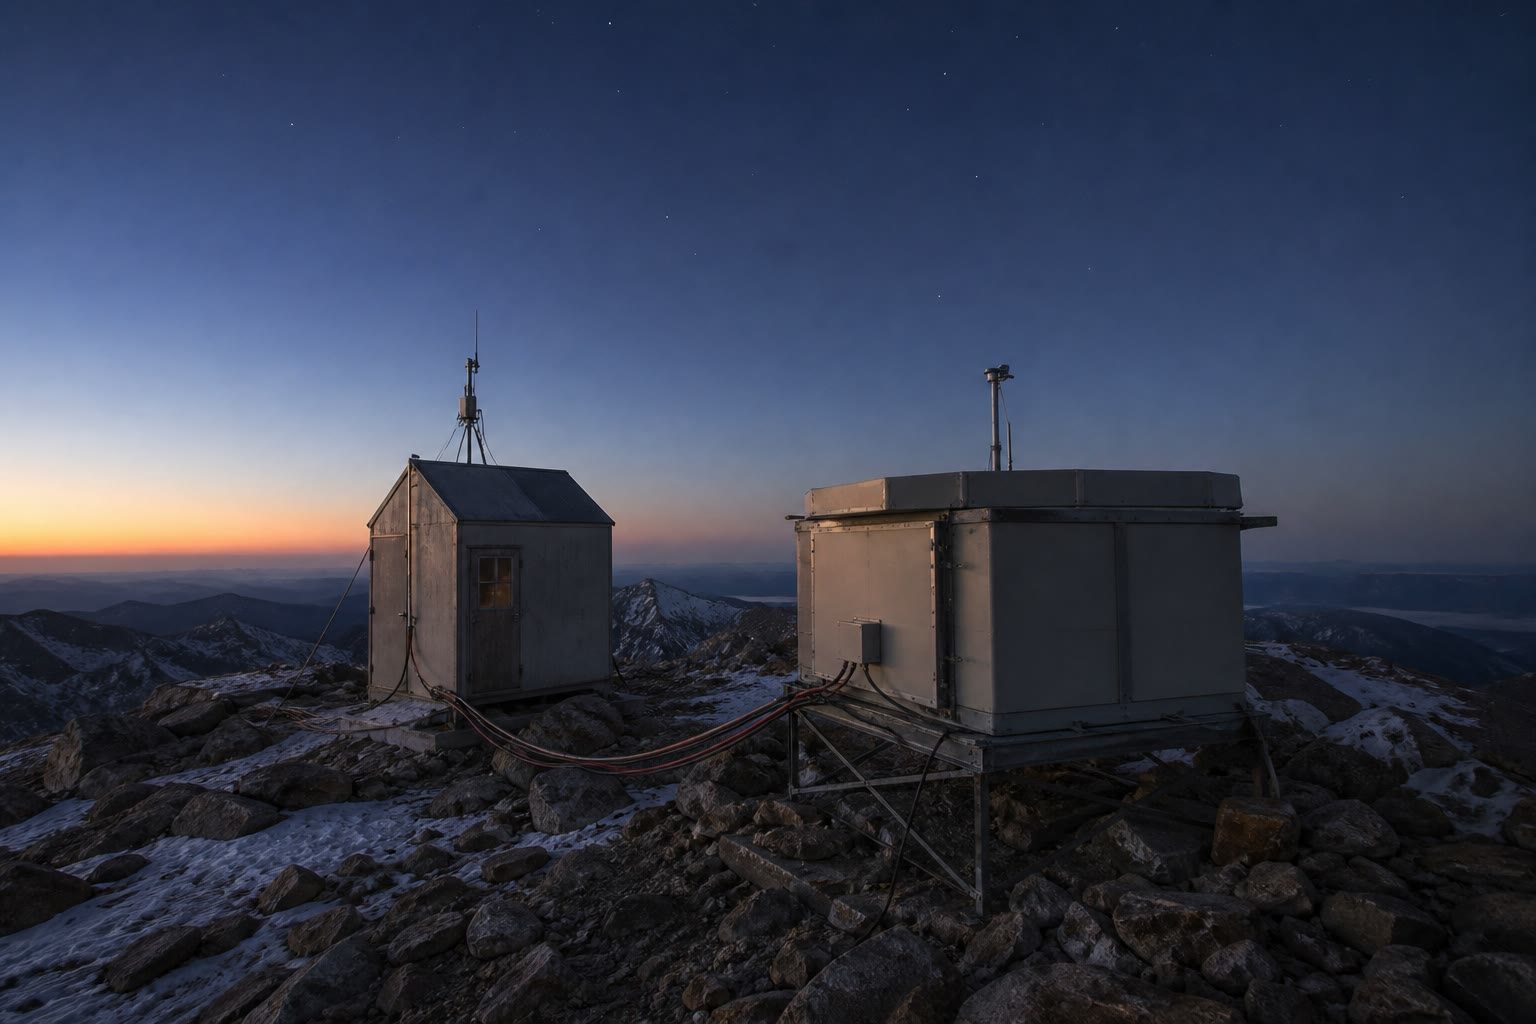
\includegraphics[width=0.58\linewidth]{images/book5/ai/b5-04-cosmic-ray-station.jpg}

{\small A cosmic-ray station at altitude. The muons it counts, born ten kilometres higher, reach it only because moving clocks run slow --- \omterm{prop:b3:relativistic-kinematics:dilation}{time dilation}, measured nightly on mountaintops.}
\end{omfigure}

\section{Exercises}

\begin{exercise}[$\star$]\label{exo:b3:relativistic-kinematics:1}
Compute $\gamma$ for $v/c = 0.1$, $0.5$, $0.9$, $0.99$, $0.999$. For
the ISS (\qty{7.7}{km/s}), compute $\gamma - 1$ using the small-speed
approximation, and the time its crew ``gains'' (or loses?) per
six-month mission relative to a clock on the ground, ignoring
gravity.
\end{exercise}

\begin{exercise}[$\star$]\label{exo:b3:relativistic-kinematics:2}
The light clock of the figure: (a) write the tick $\Delta\tau =
2d/c$ of the clock at rest ($d$ the mirror spacing); (b) from
Pythagoras in the frame where it moves at $v$, derive $\Delta t =
\gamma\Delta\tau$; (c) why does the argument require the transverse
distance $d$ to be the same in both frames? (d) Give the argument
(two identical rulers passing each other) that transverse lengths
cannot change.
\end{exercise}

\begin{exercise}[$\star$]\label{exo:b3:relativistic-kinematics:3}
A muon is created at \qty{15}{km} altitude with $v = 0.999c$. (a) Its
$\gamma$ and its mean life in our frame. (b) The mean distance it
covers. (c) The atmosphere's thickness in its frame. (d) What fraction
of such muons reaches the ground, with and without relativity (decay
law $\eu^{-t/\tau}$, $\tau = \qty{2.2}{\micro s}$)?
\end{exercise}

\begin{exercise}[$\star$]\label{exo:b3:relativistic-kinematics:4}
Two \omterm{def:b3:relativistic-kinematics:event}{events} on the $x$ axis: A at $(t = 0, x = 0)$, B at $(t =
\qty{2}{\micro s}, x = \qty{300}{m})$. (a) Compute $\Delta s^2$:
timelike or spacelike? (b) Can A cause B? (c) Find the speed of the
frame in which A and B occur at the same place, and the \omterm{prop:b3:relativistic-kinematics:dilation}{proper time}
between them there. (d) Same three questions for B at
$(\qty{1}{\micro s}, \qty{600}{m})$ --- which frame now exists, and
which does not?
\end{exercise}

\begin{exercise}[$\star\star$]\label{exo:b3:relativistic-kinematics:5}
GPS satellites orbit at $v = \qty{3.87}{km/s}$. (a) Compute $\gamma -
1$. (b) By how much does a satellite clock lag a ground clock per day,
from \omterm{prop:b3:relativistic-kinematics:dilation}{time dilation} alone? (c) Positioning works by timing signals at
$c$: what position error corresponds to one day of uncorrected
special-relativistic drift? (d) The full correction (with gravity,
treated in the final chapter's spirit) is $+38\,\unit{\micro s}$ per
day, the gravitational blueshift \emph{winning} over \omterm{prop:b3:relativistic-kinematics:dilation}{time dilation}:
what does the sign tell you about which effect is larger at
\qty{20200}{km} altitude?
\end{exercise}

\begin{exercise}[$\star\star$]\label{exo:b3:relativistic-kinematics:6}
(a) A ship at $0.8c$ launches a probe forward at $0.8c$ relative to
itself: the probe's speed for us? (b) Two ships approach each other,
each at $0.9c$ in our frame: their relative speed? (c) Show from the
composition law that $u' < c$ and $v < c$ imply $u < c$ (factor the
expression $c - u$). (d) A laser pointer swept across the face of the
Moon can paint a spot moving faster than $c$: why does this break no
law?
\end{exercise}

\begin{exercise}[$\star\star$]\label{exo:b3:relativistic-kinematics:7}
The sodium doublet at \qty{589.0}{nm} arrives from a star at
\qty{575.0}{nm}. (a) Approaching or receding? At what speed? (b) At
what speed would visible light (\qty{550}{nm}) be shifted into the
near infrared (\qty{1100}{nm})? (c) For $\beta \ll 1$, show
$\Delta\lambda/\lambda \approx \beta$ and give the rule of thumb in
km/s per \unit{\angstrom} at \qty{600}{nm}. (d) A source circling at
constant distance shows a shift even with no radial motion: which
effect is that, and of what order in $\beta$?
\end{exercise}

\begin{exercise}[$\star\star$]\label{exo:b3:relativistic-kinematics:8}
The pole and the barn. A \qty{20}{m} pole is carried at $\gamma = 2$
toward a \qty{10}{m} barn with two doors. (a) The pole's length in the
barn frame: does it fit? (b) In the runner's frame the \emph{barn} is
\qty{5}{m} long: how can both be right? Identify the two \omterm{def:b3:relativistic-kinematics:event}{events}
(``front door closes'', ``back door opens'') and compare their time
order in the two frames. (c) Compute the time between these \omterm{def:b3:relativistic-kinematics:event}{events} in
each frame for simultaneous-in-the-barn closing. (d) State the moral
in one sentence (which silent assumption did the ``paradox'' make?).
\end{exercise}

\begin{exercise}[$\star\star$]\label{exo:b3:relativistic-kinematics:9}
A rocket of \omterm{prop:b3:relativistic-kinematics:contraction}{proper length} \qty{100}{m} passes a space station at
$0.6c$. (a) How long does the station clock take between the nose's
passage and the tail's? (b) Same question for a clock on the rocket
watching the station (\omterm{prop:b3:relativistic-kinematics:contraction}{proper length} \qty{300}{m}) go by. (c) The
station fires two docking clamps simultaneously (in its frame),
\qty{80}{m} apart: what is the time between the two firings for the
rocket, and which fires first? (d) Verify $\Delta s^2$ agrees between
the frames for the pair of clamp \omterm{def:b3:relativistic-kinematics:event}{events}.
\end{exercise}

\begin{exercise}[$\star\star\star$]\label{exo:b3:relativistic-kinematics:10}
The twins, in full. Stella flies at $0.8c$ to a star \qty{8}{ly} away
(Earth frame) and returns at $0.8c$; Terra stays. (a) Compute each
twin's elapsed time. (b) In Stella's outbound frame, how far away is
the star, and how long does the outbound leg take her? (c) Just
before and just after turnaround, what does Stella compute for ``the
time now on Earth'' (use the $vx/c^2$ term)? Show her accounting jumps
by years at the kink --- and that this jump is exactly what reconciles
the totals. (d) Explain why no symmetric argument can be run from
Stella's side.
\end{exercise}

\begin{exercise}[$\star\star\star$]\label{exo:b3:relativistic-kinematics:11}
Deriving Lorentz honestly. (a) Argue from homogeneity that the
transformation must be linear. (b) Assuming $x' = \gamma(x - vt)$ and,
by the relativity principle, $x = \gamma(x' + vt')$, derive $t'$ in
terms of $t$ and $x$ without using light. (c) Show that requiring
$x = ct \Rightarrow x' = ct'$ fixes $\gamma$ to its stated value. (d)
Where exactly did the argument use each postulate?
\end{exercise}

\begin{exercise}[$\star\star\star$]\label{exo:b3:relativistic-kinematics:12}
Rapidity. Define $\varphi$ by $\tanh\varphi = \beta$. (a) Show the
\omterm{thm:b3:relativistic-kinematics:lorentz}{Lorentz transformation} reads $ct' = ct\cosh\varphi - x\sinh\varphi$,
$x' = x\cosh\varphi - ct\sinh\varphi$: a ``rotation'' by an imaginary
angle, preserving $c^2t^2 - x^2$ as rotations preserve $x^2 + y^2$.
(b) Show that composing velocities \emph{adds rapidities}: $\varphi =
\varphi_1 + \varphi_2$, and recover the composition law from
$\tanh(\varphi_1 + \varphi_2)$. (c) A rocket accelerates at $g$ in its
own frame: admitting that its rapidity grows as $\dd\varphi = g\,
\dd\tau/c$, find $\beta(\tau)$ and how much \omterm{prop:b3:relativistic-kinematics:dilation}{proper time} it takes to
reach $0.99c$. (d) Why can rapidity grow forever while $\beta$
cannot?
\end{exercise}

\begin{omfigure}
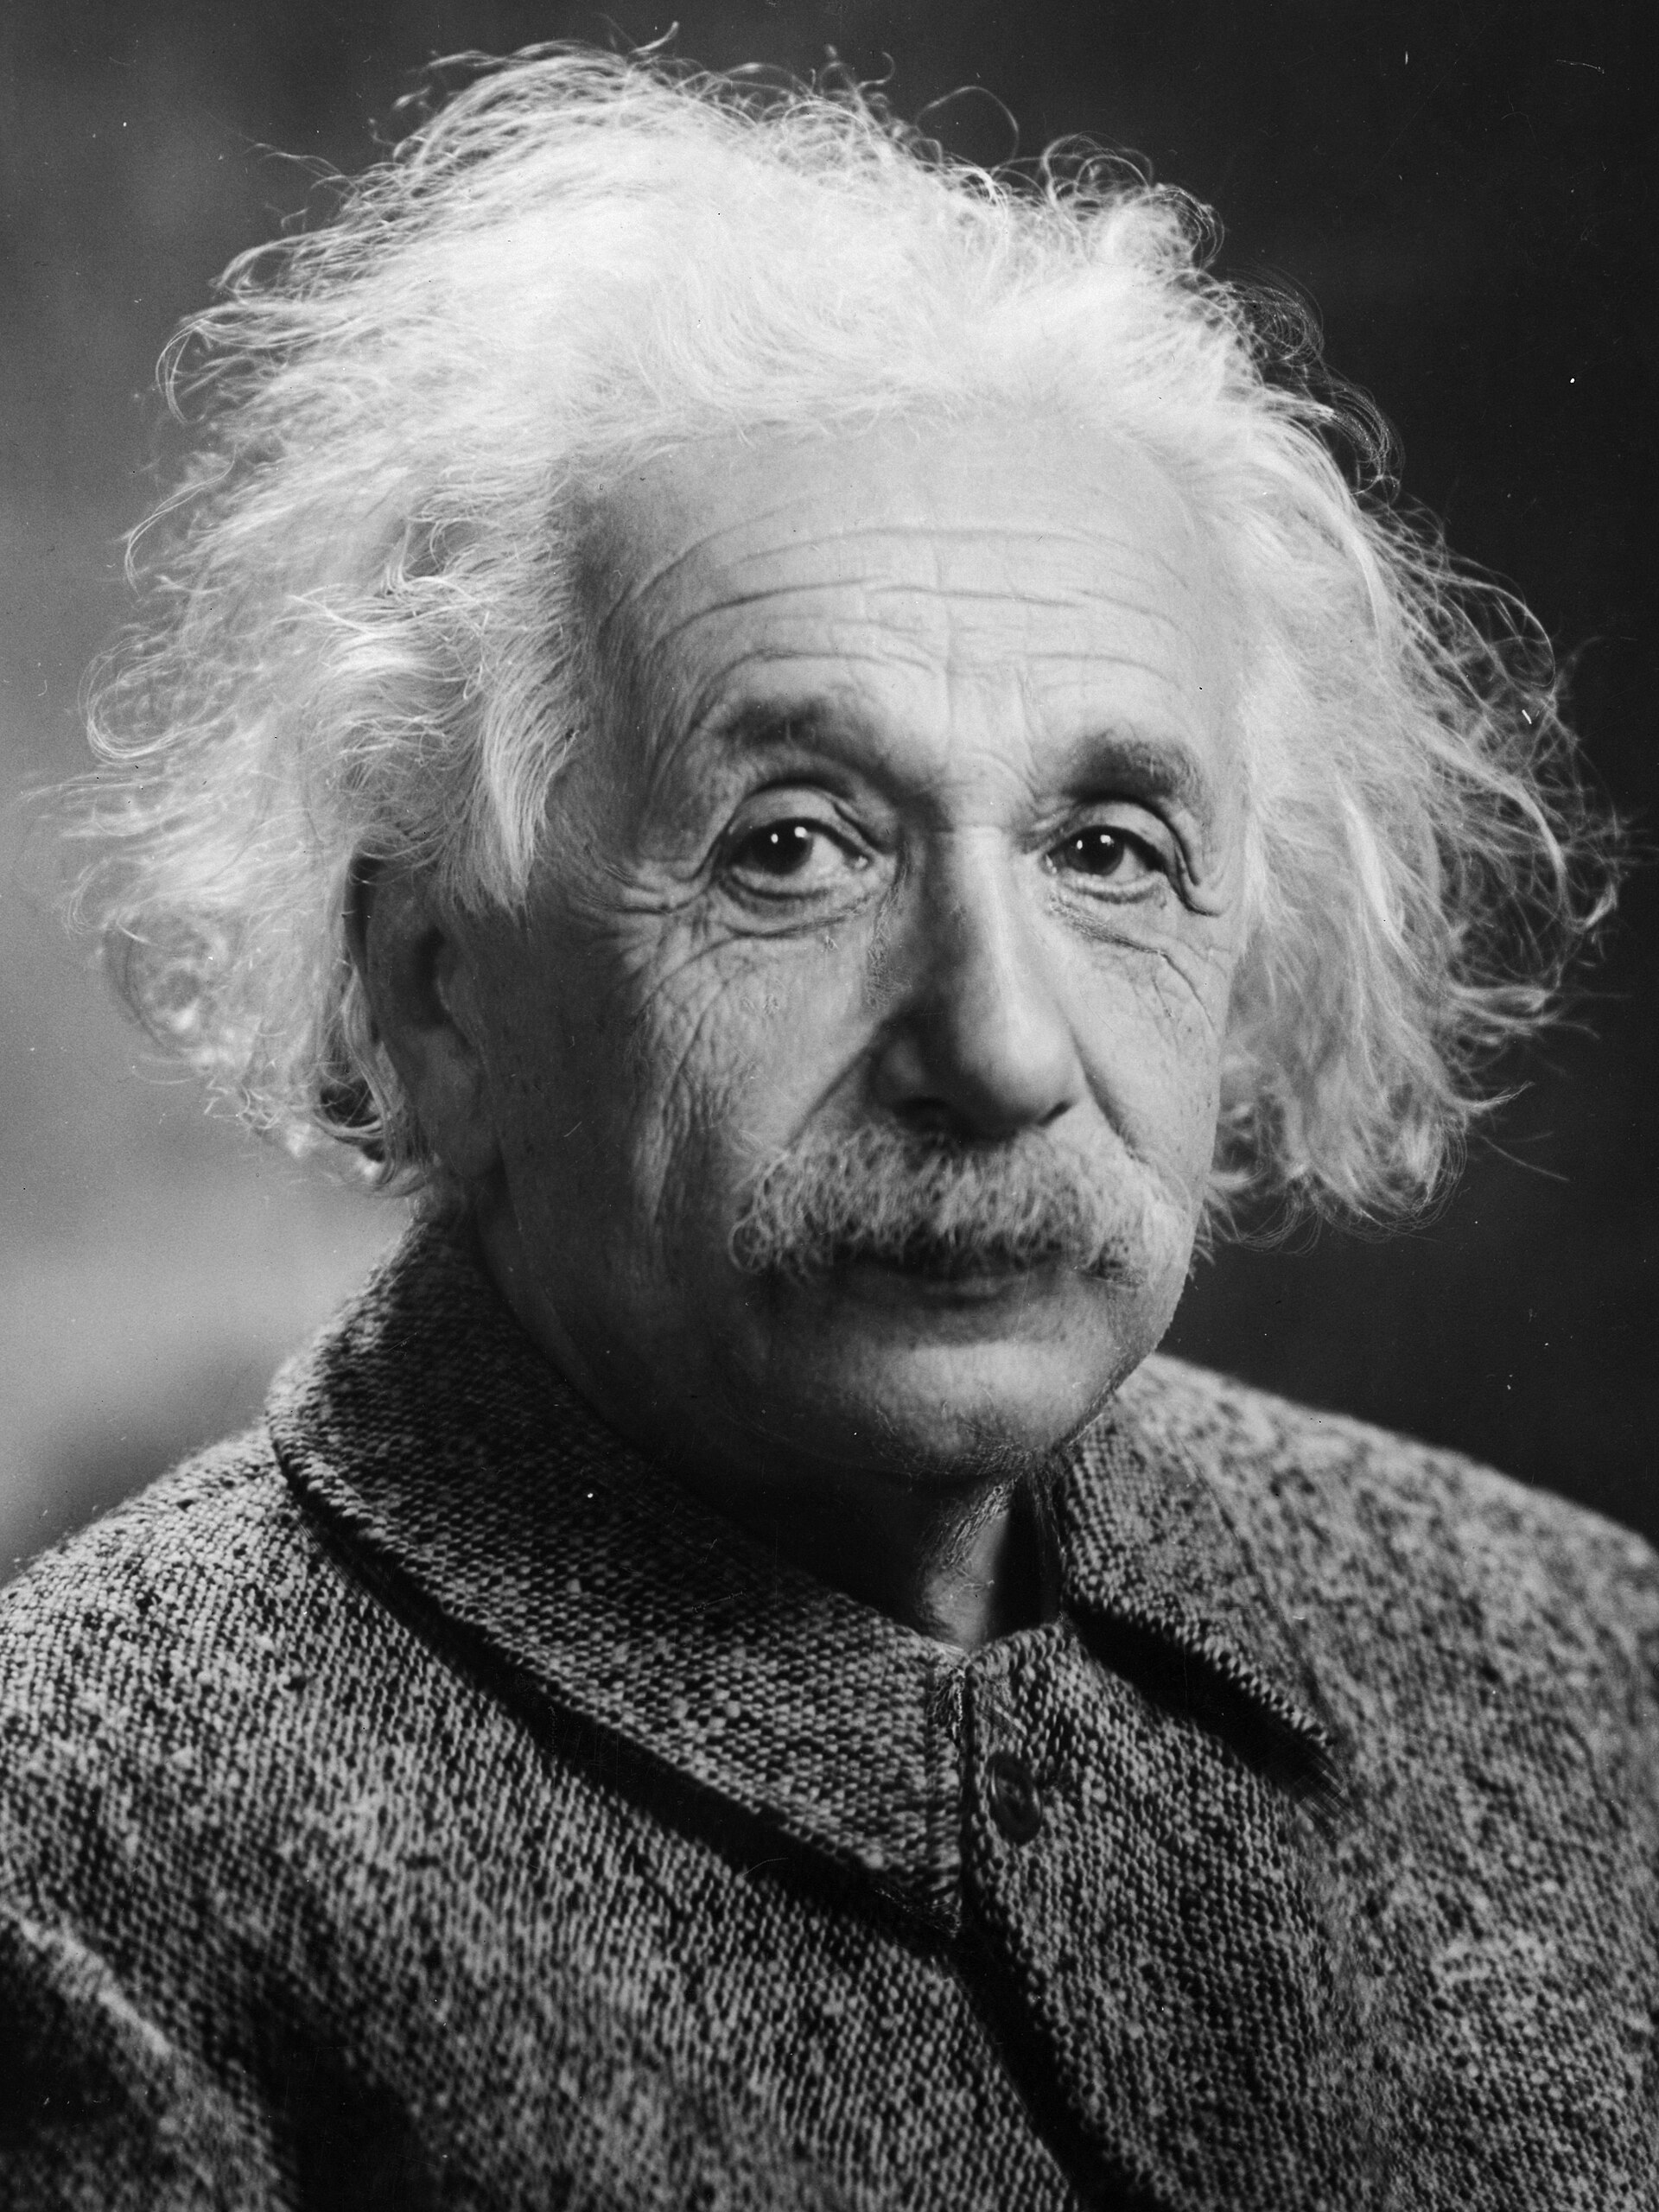
\includegraphics[width=0.34\linewidth]{images/book5/photo-einstein-1947.jpg}

{\small Albert Einstein (photograph by Orren Jack Turner, 1947, public domain). The 1905 relativity paper rebuilt kinematics from two postulates --- this chapter, essentially unchanged, is that paper with exercises.}
\end{omfigure}

\section{Problem: The experiment in the sky}

\begin{problem}[{Weekend problem --- muons, mountain clocks and the
proof that time dilates}]\label{pb:b3:relativistic-kinematics:1}
The cleanest early test of \omterm{prop:b3:relativistic-kinematics:dilation}{time dilation} used no laboratory
apparatus: nature supplies relativistic clocks by the thousand, raining
on every mountain. This problem reconstructs the Frisch--Smith
experiment (1963), then brings the same physics down to airliners and
navigation satellites. Data: muon mean proper life $\tau =
\qty{2.20}{\micro s}$; decay is exponential, a fraction
$\eu^{-t/\tau}$ of muons surviving a \omterm{prop:b3:relativistic-kinematics:dilation}{proper time} $t$; $c =
\qty{3.00e8}{m/s}$; Mount Washington: altitude difference $h =
\qty{1907}{m}$ between the two detectors.

\medskip\noindent\textbf{Part I --- Clocks that rain from the sky.}
\begin{enumerate}
  \item Cosmic protons strike nuclei high in the atmosphere and the
        debris decays into muons around \qty{15}{km} up. Why is a
        population of identical unstable particles a \emph{clock}?
  \item Compute $c\tau$, the natural range of a muon's mean life.
  \item Without relativity, what fraction of muons born at
        \qty{15}{km} and travelling at essentially $c$ would reach
        the ground? (Give the exponent; the number itself is
        absurd.)
  \item Detectors at sea level count muons abundantly: state the
        contradiction in one sentence.
  \item The sea-level flux is about one muon per square centimetre
        per minute: estimate how many muons cross your outstretched
        hand each second, and your body between two heartbeats.
  \item The experiment selected muons of speed $0.995c$: compute
        their $\gamma$.
  \item Frisch and Smith counted $563 \pm 10$ muons per hour at the
        mountaintop. Why measure at two altitudes of the \emph{same}
        shower rather than trust the \qty{15}{km} creation story?
\end{enumerate}

\medskip\noindent\textbf{Part II --- The mountain measurement.}
\begin{enumerate}[resume]
  \item How long does the trip of \qty{1907}{m} at $0.995c$ take in
        the mountain frame?
  \item Without \omterm{prop:b3:relativistic-kinematics:dilation}{time dilation}, what fraction survives that trip, and
        how many per hour should reach the bottom detector?
  \item With \omterm{prop:b3:relativistic-kinematics:dilation}{time dilation}, how much \emph{proper} time elapses for
        the muon during the trip?
  \item Predict the surviving fraction and the count per hour with
        relativity.
  \item The measured bottom count was $408 \pm 9$ per hour. Compare
        both predictions with the data, and state which theory
        survives its encounter with the mountain.
  \item From the measured ratio $408/563$, extract the
        \emph{experimental} dilation factor and compare it with
        $\gamma = 10$. (The muons slow slightly in the rock-like
        shielding, so the effective $\gamma$ is a little below the
        top-of-mountain value --- Frisch and Smith found $8.8 \pm
        0.8$.)
\end{enumerate}

\medskip\noindent\textbf{Part III --- The muon's own story.}
\begin{enumerate}[resume]
  \item In the muon's frame, how tall is Mount Washington?
  \item How long does the mountain take to stream past, and what
        fraction of muons decays in that time? Check it matches
        Part II's prediction.
  \item The two frames disagree about what dilated (our time?\ its
        mountain?) yet agree on the count: which kind of quantity is
        the count, and why must all frames agree on it?
  \item Compute the interval $\Delta s^2$ between creation at the top
        and arrival at the bottom, in the mountain frame, and check
        that $\Delta s/c$ equals the muon's \omterm{prop:b3:relativistic-kinematics:dilation}{proper time} of Part II.
  \item A sceptic objects: ``maybe altitude, not speed, changes decay
        rates.'' What control does the measured $\gamma$-dependence
        (slower muons dilate less) provide?
  \item Modern storage rings hold muons at $\gamma = 29.3$ and
        measure lifetimes to $\num{e-3}$: what do they find, and what
        does a circular orbit add to the test (which twin is the
        muon)?
\end{enumerate}

\medskip\noindent\textbf{Part IV --- Down to Earth: planes and
satellites.}
\begin{enumerate}[resume]
  \item An airliner cruises at \qty{250}{m/s} for a \qty{40}{h}
        round-the-world flight. Using $\gamma - 1 \approx v^2/2c^2$,
        compute the special-relativistic lag of its clock, in
        nanoseconds.
  \item Caesium clocks resolve nanoseconds easily; the 1971 flights
        confirmed the prediction (once gravity's opposite push,
        larger at altitude, was included). Why must the two effects
        be separated by flying \emph{both} eastward and westward?
  \item A GPS satellite ($v = \qty{3.87}{km/s}$) accumulates what
        special-relativistic clock lag per day, in microseconds?
  \item Uncorrected, how many kilometres of ranging error would
        \emph{one week} of that drift alone produce?
  \item The complete GPS correction, $+38\,\unit{\micro s}$ per day
        with gravity included, is engineered into the satellite
        clocks before launch: what would a navigator observe within
        hours if it were not?
  \item Summarise the named result: a mountain, two counters and
        $2.2\,\unit{\micro s}$ clocks measured \omterm{prop:b3:relativistic-kinematics:dilation}{time dilation} at
        $\gamma \approx 9$ within $10\%$ in 1963 --- and the same
        physics is corrected for, every second, in every phone that
        knows where it is.
\end{enumerate}
\end{problem}
